\section{Progettazione}

% 2.2.1
\subsection{Costruzione degli scenari}
Prima di analizzare le scelte attuate nella progettazione dei pedoni, è doveroso porre l'attenzione sugli elementi caratterizzanti lo scenario nel quale questi devono essere inseriti, in modo da capire come gli elementi appartenenti al modello di Alchemist, sono stati ampliati o adattati per essere utilizzati nel contesto dell'evacuazione di folle. 

\subsubsection{Ambienti}
Pur essendo presenti molte tipologie di ambiente in Alchemist, nessuno di questi presentava una componente fisica che si occupasse di gestire la forma geometrica dei vari nodi, al fine di impedire che questi si presentassero contemporaneamente nella stessa porzione di spazio. \newline
Questa limitazione non permetteva il verificarsi di fenomeni molto comuni, come l'accalcamento di pedoni in prossimità dell'uscita o l'intralcio nel movimento dovuto all'alta densità di persone perché, consentendo la sovrapposizione, nessun individuo poteva essere ostacolato nelle sue azioni dalla presenza degli altri. \newline
Per questo motivo, è stato introdotto il concetto di \texttt{PhysicsEnvironment}, un ambiente nel quale il movimento o il cambiamento di orientamento di un nodo è vincolato dalla non collisione con nessun altro nodo all'interno di esso. \newline
Visti gli svariati campi applicativi in cui questa soluzione si potrebbe rivelare utile, si è deciso di ristrutturare la gerarchia preesistente degli ambienti, che ora si presenta come in figura \ref{fig:environments-uml}, dove le nuove interfacce e classi inserite sono state contrassegnate con un colore leggermente più scuro.

\begin{figure}[ht]
  \centering
  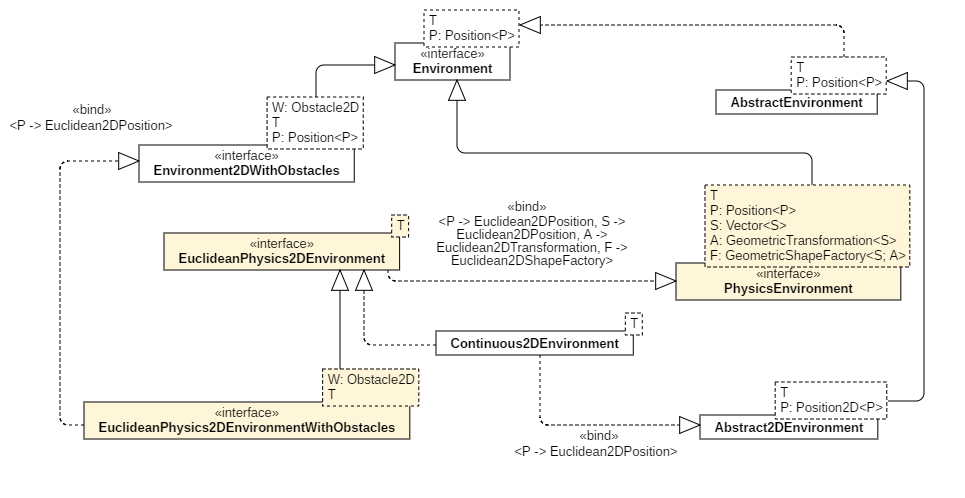
\includegraphics[width=1.0\linewidth]{immagini/uml/environments.png}
  \caption{Nuovo diagramma delle classi in UML degli ambienti in Alchemist.}
  \label{fig:environments-uml}
\end{figure}

\subsubsection{Punti di interesse}
Il solo ambiente non è sufficiente a descrivere lo scenario di interesse nel caso di un'evacuazione, infatti, è essenziale che vi sia un modo per poter rappresentare i pericoli da cui si sta scappando e i punti da raggiungere per mettersi in salvo. \newline
Per definire queste zone, è stata associata ad ognuna di esse una molecola identificativa e ci si è avvalsi dell'uso dei \texttt{Layer}, strati costitutivi la distribuzione spaziale della concentrazione di una determinata molecola all'interno dell'ambiente. \newline 
Nello specifico, sono stati utilizzati dei \texttt{BidimensionalGaussianLayer}, livelli caratterizzati da una distribuzione gaussiana delle concentrazioni, modulabili attraverso la regolazione di intensità e ampiezza per rappresentare tanto un fiammifero acceso quanto un incendio divampato. \newline
La scelta della tipologia di \texttt{Layer} è assolutamente indipendente dall'ambiente che si sta utilizzando, quindi, è possibile definire a proprio piacimento la struttura spaziale che si intende ottenere per modellare fenomeni anche meno localizzati e più irregolari rispetto a quelli sopra citati.

% 2.2.2
\subsection{Pedoni omogenei, eterogenei e cognitivi}
Partendo dal concetto di nodo in Alchemist, piuttosto che creare un unico onnicomprensivo modello di pedone, la decisione è stata di procedere analizzando tre livelli crescenti di dettaglio, nello specifico:
\begin{itemize}
    \item \textbf{Pedone omogeneo}: un nodo con una velocità predefinita di camminata e di corsa uguale per tutti.
    \item \textbf{Pedone eterogeneo}: un nodo con un sesso ed una età assegnati, dai quali saranno determinate velocità, conformità alle regole ed attitudine ad aiutare.
    \item \textbf{Pedone cognitivo}: un pedone eterogeneo con delle emozioni, capace di influenzare e farsi influenzare dagli altri.
\end{itemize}
Questo approccio rende possibile confrontare, ripetendo la stessa simulazione con tutte e tre le tipologie di pedone, il comportamento delle diverse astrazioni, in modo da valutare la rilevanza di determinate caratteristiche.
\newline
Per ogni genere di pedone, è stato definito un prototipo di base con l'obiettivo di incapsulare la gestione delle caratteristiche ad esso inerenti al suo interno. La modellazione di aspetti più strettamente collegati all'ambiente di simulazione che si sta utilizzando, come la struttura fisica, viene invece delegata a eventuali classi create estendendo tali prototipi, in modo da rendere il più agevole possibile il loro utilizzo anche in previsione di eventuali ambientazioni tridimensionali o non governate dalle leggi della geometria euclidea. \newline
Il diagramma delle classi rappresentante la struttura dei vari pedoni è presentato in figura \ref{fig:pedestrians-uml}.

\begin{figure}[ht]
  \centering
  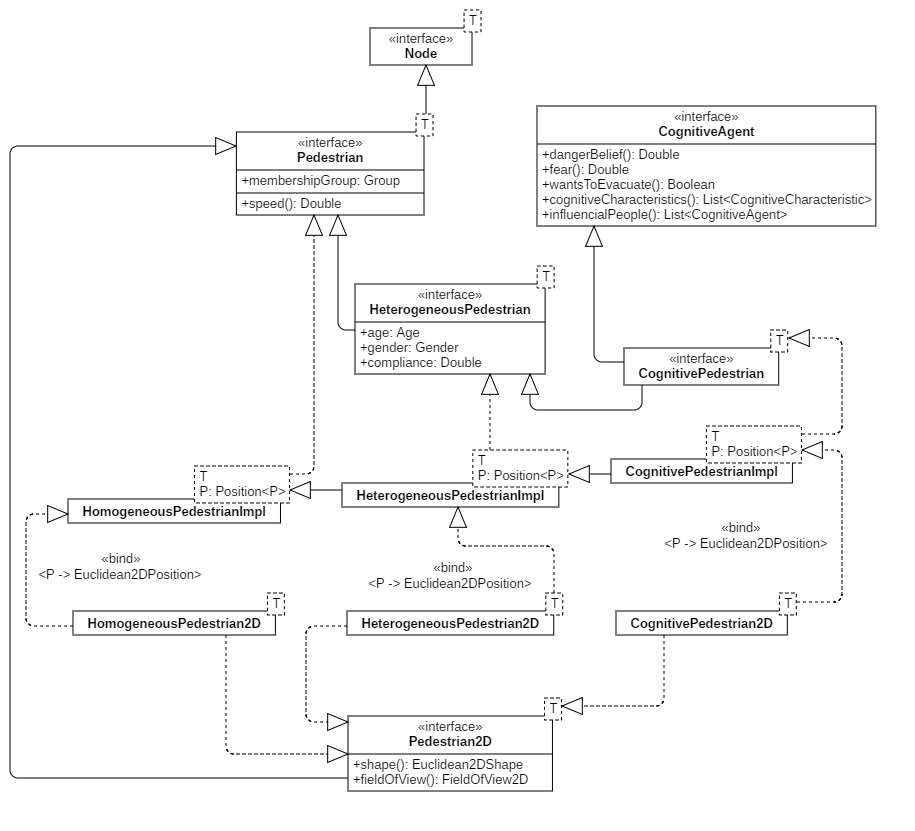
\includegraphics[width=0.8\linewidth]{immagini/uml/pedestrians.png}
  \caption{Diagramma delle classi in UML delle varie tipologie di pedone.}
  \label{fig:pedestrians-uml}
\end{figure}

\subsubsection{Pedoni bidimensionali}
Non avendo Alchemist attualmente a disposizione delle funzionalità per la simulazione tridimensionale, la concentrazione è stata focalizzata sulla creazione di pedoni bidimensionali, realizzati per ognuna delle tre categorie precedentemente descritte. \newline
Questi pedoni, la cui forma è stata approssimata a quella di un cerchio, hanno sia il vincolo di dover essere inseriti in un \texttt{EuclideanPhysics2DEnvironment}, un ambiente caratterizzato da una componente fisica e governato dalle leggi della geometria euclidea, sia la restrizione di poter essere equipaggiati solamente con delle sfere di influenza bidimensionali, come il \texttt{FieldOfView2D}. \newline
Nonostante questa scelta possa sembrare limitativa, garantisce la consistenza tra i vari elementi all'interno della simulazione ed esplicita immediatamente gli scenari in cui è idoneo utilizzare questa tipologia di nodo.

% 2.2.3
\subsection{Fenomeni cognitivi}
Per una migliore organizzazione, si è deciso di suddividere le caratteristiche inerenti i pedoni in due categorie a seconda della loro funzione:
\begin{itemize}
    \item \textbf{Caratteristiche individuali}: intrinsecamente parte del pedone e non mutabili nel corso della simulazione. Appartengono a questa categoria: età, sesso, velocità, conformità alle regole, ed attitudine ad aiutare.
    \item \textbf{Caratteristiche cognitive}: costitutive della componente relazionale ed emotiva del pedone e variabili nel corso della simulazione. Appartengono a questa categoria: sensazione di pericolo, paura, desiderio di fuggire e di non fuggire, intenzione di fuggire e di non fuggire.
\end{itemize}
Tale suddivisione ha permesso di sfruttare, nel caso delle caratteristiche cognitive, i vantaggi del pattern comportamentale \textit{template method} \cite{GoF1995}, illustrato in figura \ref{fig:cognitive-characteristics-uml}, con il quale sono state ristrutturate le equazioni differenziali relative ad ogni caratteristica. Ad ognuna di esse è stata associata solamente la relativa funzione di combinazione $c_{y}$ ed è stato così ridotto il rischio di errore in fase di implementazione, ma anche il grado di difficoltà di comprensione in caso di futura modifica. \newline
Per quanto riguarda la gestione dell'evoluzione dei processi emotivi, è stata creata una reazione responsabile di questo tipo di comportamenti, incaricata di risolvere per ogni emozione considerata, l'equazione ad essa relativa. \newline
Le caratteristiche inerenti i pedoni sono state modellate in maniera completamente indipendenti dalla struttura di Alchemist, con l'obiettivo di poterle estrapolare e riutilizzare anche in altri contesti applicativi.

\begin{figure}[ht]
  \centering
  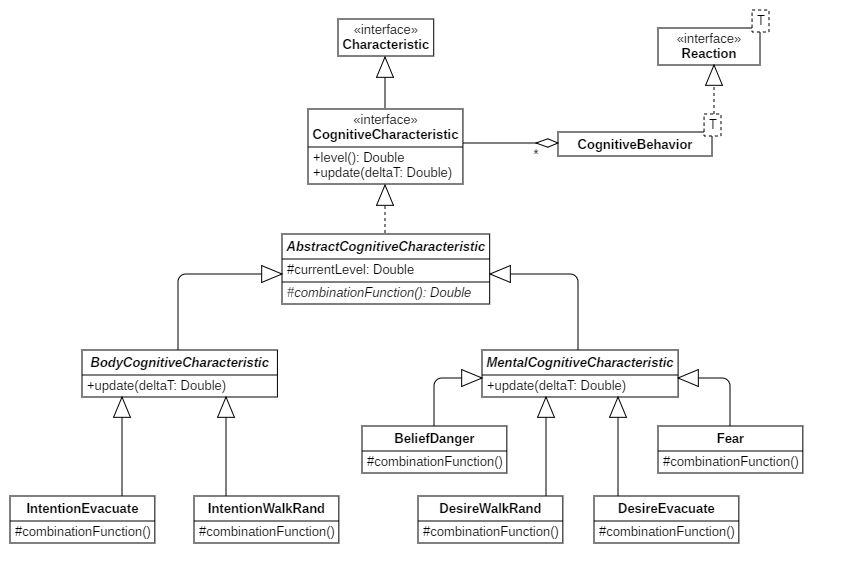
\includegraphics[width=0.8\linewidth]{immagini/uml/cognitive-characteristics.png}
  \caption{Diagramma delle classi in UML delle caratteristiche cognitive di un agente.}
  \label{fig:cognitive-characteristics-uml}
\end{figure}

% 2.2.4
\subsection{Comportamenti di steering}
É stata utilizzata come punto di partenza l'azione \texttt{AbstractConfigurableMoveNode}, che permette di scegliere il punto di arrivo, la rotta da seguire e la velocità alla quale procedere. Si è arrivati così a definire un'implementazione comune ai vari comportamenti di steering. \newline
Al fine di non vincolare al mondo euclideo questi aspetti, che potrebbero essere utilizzati anche in ambiti dove tale geometria non è valida, si è deciso di mantenere generica la tipologia di posizione utilizzata. Un esempio è quello del traffico stradale, dove ad una vettura non è sempre concesso proseguire in entrambi i sensi di marcia. \newline
Per rappresentare il flusso da seguire, si è fatto uso di \texttt{Layer} e sono state emulate le direzioni costituenti il campo vettoriale sfruttando la differenza di concentrazione della molecola ad esso associata, tra due diversi punti dello spazio. Grazie a questa scelta, il pedone può essere alternativamente mosso verso posizioni contraddistinte da un gradiente sempre maggiore o da uno sempre minore. \newline
Oltre alle azioni di steering formulate da Reynolds, ne è stata introdotta una denominata \texttt{Combine}, responsabile di determinare la rotta finale da far seguire al pedone combinando quelle di tutte le altre presenti.

\begin{figure}[ht]
  \centering
  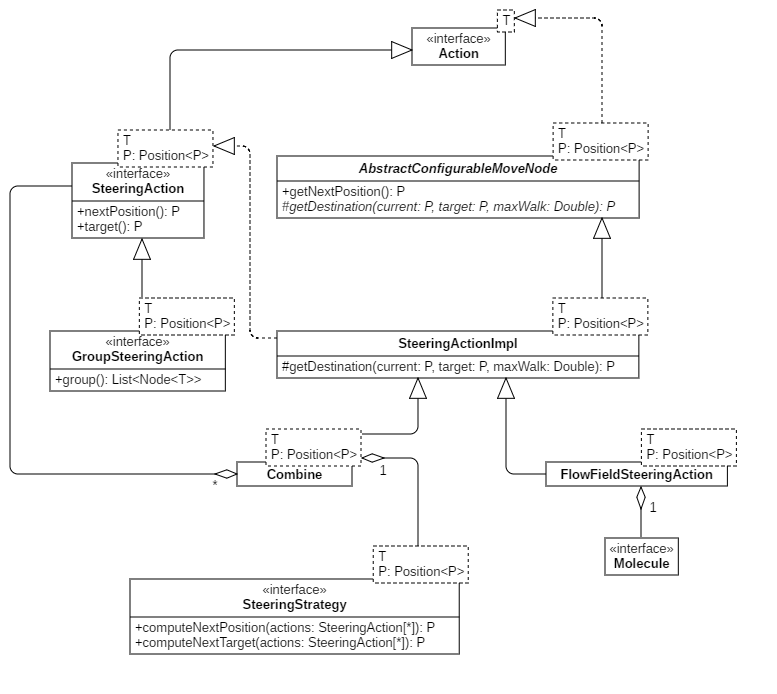
\includegraphics[width=0.8\linewidth]{immagini/uml/steering-actions.png}
  \caption{Diagramma delle classi in UML della struttura delle azioni di steering.}
  \label{fig:steering-actions-uml}
\end{figure}

% 2.2.5
\subsection{Strategie di steering}
Il movimento dei pedoni, pur differenziandosi in relazione alle caratteristiche associate ad ognuno di essi, consiste sempre nella combinazione di multiple azioni di steering, che determinano la direzione da seguire al fine di conseguire tutti gli obiettivi prefissati. \newline
Cercando di realizzare questo principio, attraverso la somma vettoriale delle varie forze di steering tuttavia, è possibile incorrere in problemi di stallo o movimenti impredicibili, dovuti all'inibizione o addirittura all'annullamento di forze che, per motivi strutturali, sono una l'opposto dell'altra. \newline
Per differenziare l'attitudine del pedone a compiere una determinata azione piuttosto che un'altra sono state formulate delle strategie, algoritmi attraverso i quali modificare il modulo delle forze valutate per aumentarne o diminuirne l'influenza nel calcolo della direzione finale. \newline 
Il modulo della forza risultante è irrilevante ai fini della rapidità di spostamento del pedone, che è invece determinata dalla sua velocità. \newline 
Non essendovi delle regole ben precise per calcolare la rilevanza di ogni forza rispetto alle altre e dipendendo tale calcolo anche dallo scenario preso in considerazione, si è mantenuta la modellazione il più generale possibile. \newline 
In particolare sono state formulate alcune strategie di esempio, in modo da fornire una base di partenza per la creazione di eventuali altre:

\begin{itemize}
    \item \textbf{Basata sul peso}: Ad ogni azione viene associato un peso con una funzione di mapping e viene poi eseguita la somma vettoriale pesata. 

    \item \textbf{Basata sulla distanza}: Utilizza come metrica per determinare il peso di una azione di steering, la distanza tra il punto designato come da raggiungere in essa e la posizione attuale del pedone.

    \item \textbf{Massima vicinanza}: Valuta solo l'azione di steering che, considerata la posizione attuale del pedone, è quella con il punto da raggiungere più vicino ad essa.

    \item \textbf{Basata sul tipo}: Utilizza come metrica per determinare il peso, un valore associato ad ogni tipologia di azione di steering, grazie al quale, ad esempio, è possibile enfatizzare l'importanza della fuga dal pericolo, piuttosto che quella del movimento casuale.
\end{itemize}

Per massimizzare il riutilizzo delle varie logiche di steering, si è fatto uso del pattern strutturale \textit{decorator} \cite{GoF1995} creando una strategia \texttt{Filtered} con l'obiettivo di utilizzare una stessa logica su un più ristretto numero di azioni. Lo schema relativo alla struttura adottata è mostrato in figura \ref{fig:steering-strategies-uml}. \newline
Per eseguire le azioni di steering in combinazione tra loro e non una di seguito all'altra, ha avuto un ruolo decisivo la realizzazione della reazione \texttt{SteeringBehavior}, capace di riconoscere ed eseguire congiuntamente solo questo tipo di azioni tra tutte le varie presenti. Per permettere di scegliere al momento della scrittura della simulazione la strategia di steering da utilizzare, è stato sfruttato il pattern comportamentale \textit{strategy} per definire versioni più specifiche di questa reazione. \newline 
In particolare, a fine esemplificativo, sono stati differenziati un \texttt{PrioritySteering}, per indicare l'uso della strategia di massima vicinanza ed un \texttt{BlendedSteering}, per indicare l'uso della logica basata sulla distanza.

\begin{figure}
  \centering
  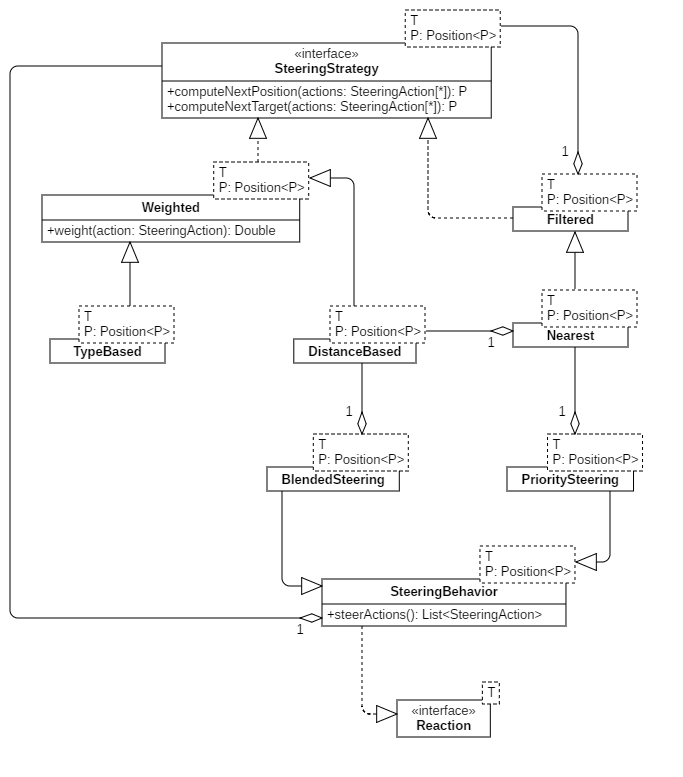
\includegraphics[width=0.75\linewidth]{immagini/uml/steering-strategies.png}
  \caption{Diagramma delle classi in UML delle strategie di steering e dei relativi comportamenti.}
  \label{fig:steering-strategies-uml}
\end{figure}

% 2.2.6
\subsection{Appartenenza ad un gruppo}
Non essendo presente un concetto analogo a quello di gruppo in Alchemist, si è deciso di introdurlo generalizzandolo per qualsiasi tipologia di nodo, in modo da poterlo impiegare anche in contesti non esplicitamente inerenti i pedoni, quali quelli del mondo animale. \newline
Per favorire l'assegnamento del gruppo di appartenenza durante il caricamento della simulazione, nello specifico durante la creazione dei nodi, viene lasciata la possibilità di aggiungere o rimuovere dei membri al suo interno. \newline
Nei gruppi in cui un elemento assume il ruolo di leader, per decidere quale membro in particolare sia degno di questo incarico, si è utilizzato un comparatore, grazie al quale è possibile usare la logica che più si ritiene opportuna per selezionare un nodo piuttosto che un altro. \newline 
Essendo questo lavoro incentrato sulle persone, le tipologie di gruppo presentate come esempio sono: \texttt{Alone} per indicare il caso limite di un pedone solitario, \texttt{Friends} per un generico insieme in cui ogni membro ha le stesse responsabilità degli altri e \texttt{Family} in modo da fornire anche un riscontro pratico alla presenza di leader. \newline
La struttura risultante è schematizzata in figura \ref{fig:groups-uml}.

\begin{figure}[ht]
  \centering
  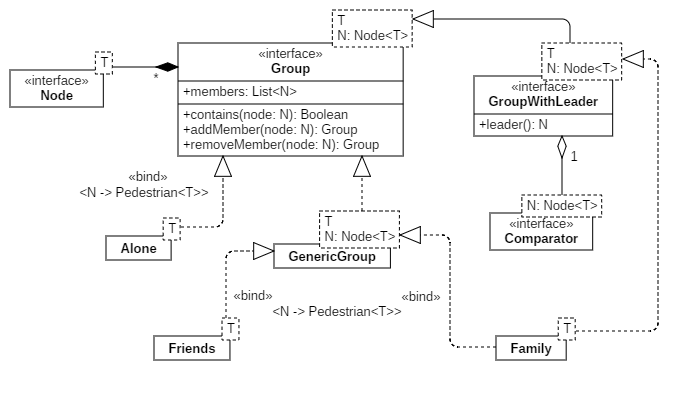
\includegraphics[width=0.75\linewidth]{immagini/uml/groups.png}
  \caption{Diagramma delle classi in UML dei gruppi.}
  \label{fig:groups-uml}
\end{figure}